% Compile twice!
% With the current MiKTeX, you need to install the beamer, and the translator packages directly form the package manager!

\documentclass{beamer}

\geometry{paperwidth=160mm,paperheight=160mm}

\usepackage{tikz}
\usetikzlibrary{shapes,arrows}

\usepackage[T1]{fontenc}
\usepackage{amsfonts}
\usepackage{amsmath}
\usepackage[utf8]{inputenc}

\usetheme{boxes}

% tikz settings for the flowchart(s)

\tikzstyle{decision} = [diamond, minimum width=3cm, minimum height=1cm, text centered, draw=black, fill=green!15]
\tikzstyle{block} = [rectangle, draw, fill=blue!15, text width=20em, text centered, minimum height=1em]
    
\tikzstyle{line} = [draw, -latex']
\tikzstyle{cloud} = [draw, ellipse,fill=red!20, node distance=3cm,
    minimum height=2em]
\tikzstyle{arrow} = [thick,->,>=stealth]

\begin{document}

\begin{frame}[plain]
\begin{tikzpicture}[overlay, remember picture]
\node[anchor=center] at (current page.center) {
\begin{beamercolorbox}[center]{title}
    {\Huge A Számítástudomány Alapjai I}\\
    {\Large Vizsgatételek}
\end{beamercolorbox}};
\end{tikzpicture}
\end{frame}

% --------------------  LOGIKA --------------------

\begin{frame}[plain]
\begin{tikzpicture}[overlay, remember picture]
\node[anchor=center] at (current page.center) {
\begin{beamercolorbox}[center]{title}
    {\Huge Logika}
\end{beamercolorbox}};
\end{tikzpicture}
\end{frame}


\begin{frame}

\begin{block}{Tétel: Minden formula egyértelműen olvasható}
F formulára a következő állítások közül pontosan egy teljesül:

\begin{enumerate}
\item F egy változó.
\item Pontosan egy G formulára $F = \neg G$
\item Pontosan egy G és pontosan egy H formuláta $F = (G \land H)$
\item Pontosan egy G és pontosan egy H formulára $F = (G \lor H)$
\end{enumerate}

\end{block}

\end{frame}


\begin{frame}

\begin{block}{Tétel: Az ítéletkalkulus kompaktsági tétele}
Egy formulahalmaz akkor és csak akkor elégíthető ki, ha minden véges részhalmaza kielégíthető.

\end{block}

\begin{block}{Tétel: Adekvát halmazok}
$\{\neg, \lor, \land\}, \{\neg, \lor\}, \{\neg, \land\}$ adekvát (azaz bármilyen formula leírható ezekkel), $\{\lor, \land\}$ nem adekvát.

\end{block}

\end{frame}


\begin{frame}

\begin{block}{tétel: Equivalens állítások formulákra}
Legyenek $F, F_1, ... , F_n$ tetszőleges formulák, ekkor a következő állítások equivalensek:

\begin{enumerate}
\item $\{F_1, ... , F_n\} \models F$
\item $F_1 \land ... \land F_n \implies F$ tautológia
\item $F_1 \land ... \land F_n \land \neg F$ kielégíthetetlen.
\end{enumerate}

\end{block}

\end{frame}

\begin{frame}

\begin{block}{Lemma: Helyettesítési Lemma}
Legyenek $F, G, H$ formulák úgy, hogy $F \equiv G$ és $F$ a $G$ részformulája.\\
Ha $H[F/G]$ azt a formulát jelöli, amelyben $F$ valamely előfordulását helyettesítettük $G$-vel, akkor
$$H \equiv H[F/G]$$

\end{block}

\end{frame}


\begin{frame}

\begin{block}{Tétel: Konjunktív és diszjunktív normálforma létezése}
Minden $F$ Formulához létezik vele logikailag ekvivalens konjunktív és diszjunktív normálforma.

\end{block}

\begin{block}{Bizonyítás}
Konjunktív:
\begin{enumerate}
	\item (Negáció bevitele.) Amíg lehetséges, helyettesítsük $F$-ben a
	\begin{itemize}
		\item $\neg \neg G$ alakú részformulákat $G$-vel,
		\item $\neg (G \land H)$ alakú részformulákat $\neg G \lor \neg H$-val,
		\item $\neg (G \lor H)$ alakú részformulákat $\neg G \land \neg H$-val.
	\end{itemize}
	\item Amíg lehetséges, helyettesítsük $F$-ben a
	\begin{itemize}
		\item $F \lor (G \land H)$ alakú részformulákat $(F \lor G) \land (F \lor H)$-val,
		\item $(F \land G) \lor H$ alakú részformulákat $(F \lor H) \land (G \lor H)$-val.
	\end{itemize}
\end{enumerate}

Diszjunktív:
\begin{enumerate}
	\item Ugyanaz mint a konjunktív normálforma esetén.
	\item Amíg lehetséges, helyettesítsük $F$-ben a
	\begin{itemize}
		\item $F \land (G \lor H)$ alakú részformulákat $(F \land G) \lor (F \land H)$-val,
		\item $(F \lor G) \land H$ alakú részformulákat $(F \land H) \lor (G \land H)$-val.
	\end{itemize}
\end{enumerate}
\end{block}

\end{frame}

\begin{frame}

\begin{block}{Tétel: Dedukció tétel}
Tetszőleges $\Sigma$ formulahalmaz esetén $\Sigma \vdash F \rightarrow G$ akkor és csak akkor teljesül, ha $\Sigma \cup \{F\} \vdash G$.

\end{block}

\begin{block}{Tétel: Dichotómia tétel}
Tetszőleges $\Sigma$ formulahalmaz esetén, ha $\Sigma \cup \{F\} \vdash$ (levezethető) $G$ és $\Sigma \cup \{\neg F\} \vdash G$, akkor $\Sigma \vdash G$.\\
("Az $F$ Formula nem szól bele").

\end{block}

\begin{block}{Tétel: Helyességi tétel}
Tetszőleges $\Sigma$ és $F$ esetén, ha $\Sigma \vdash F$, akkor $\Sigma \models F$.\\
(Helyes, ha csak az elélethez tartozó formulákat lehet bizonyítani.)

\end{block}

\begin{block}{Tétel: Teljességi tétel}
Minden $\Sigma$-ra és $F$-re, ha $\Sigma \models F$, akkor $\Sigma \vdash F$.\\
(Teljes, ha minden, az elmélethez tartozó formulát be lehet bizonyítani.)

\end{block}

\begin{block}{Tétel: Konzisztencia tétel}
Tetszőleges formulahalmaz, akkor és csak akkor konzisztens, ha kielégíthető.\\
(Konzisztens, ha nem vezethető le belőle a $\downarrow$.)

\end{block}

\end{frame}

% --------------------  GRÁFELMÉLET --------------------

\begin{frame}[plain]
\begin{tikzpicture}[overlay, remember picture]
\node[anchor=center] at (current page.center) {
\begin{beamercolorbox}[center]{title}
    {\Huge Gráfelmélet}
\end{beamercolorbox}};
\end{tikzpicture}
\end{frame}


\begin{frame}

\begin{block}{Tétel: Fokszám-Élszám}
Legyen $G = (V, E)$ (Gráf). Ekkor $G$-ben a páratlan fokú csúcsok száma páros.

\end{block}

\begin{block}{Bizonyítás}
$$\sum_{a \in V} d(a) = \sum_{d(a) \equiv 0 (mod 2)} d(a) + \sum_{d(a) \equiv 1 (mod 2)} \equiv 0 (mod 2)$$
amiből kapjuk, hogy $$\sum_{d(a) \equiv 1 (mod 2)} d(a) \equiv 0 (mod 2)$$.

\end{block}

\end{frame}

\begin{frame}

\begin{block}{Tétel: Equivalens állítások fákra}
Egy $G$ egyszerű gráfra a következő állítások equivalensek:

\begin{enumerate}
\item $G$ Fa
\item $G$ Összefüggő, de bármely él elhagyásával kapott részgráf már nem összefüggő.
\item Ha $v, v'$ a $G$ különböző csúcsai, akkor pontosan egy út vezet $v$-ből $v'$be.
\item $G$-ben nincs kör, de bármely új él hozzáadásával kapott gráf már tartalmaz kört.
\end{enumerate}

\end{block}


\begin{block}{Tétel: Elsőfokú pontok}
Ha egy véges gráfban nincs kör, de van él, akkor van benne legalább két elsőfokú pont.

\end{block}

\end{frame}

\begin{frame} 

\begin{block}{Tétel: Ekvivalens állítások n-pontú fákra}
Egy $G$ egyszerű gráfra a következő álítások ekvivalensek:

\begin{enumerate}
\item $G$ fa.
\item $G$-ben nincs kör és $n - 1$ éle van.
\item $G$ összefüggő és $n - 1$ éle van.
\end{enumerate}

\end{block}

\begin{block}{Tétel: Feszítőfa létezése}
Minden véges összefüggő $G$ gráfnak létezik feszítőfája.

\end{block}

\end{frame}

\begin{frame} 

\begin{block}{Tétel: Körök száma}
Egy véges összefüggő $G = (E, V)$ gráfban létezik \underline{legalább} $e(G) - v(G) + 1$ különböző kör.

\end{block}

\begin{block}{Bizonyítás}
A feszítőfa létezése téltel miatt ($\Rightarrow$) $\exists T$ feszítőfa, aminek $v(G) - 1$ éle van.\\
Legyen $K_f$ az a kör, ami $T \cup \{f\}$-ben van, ahol $f \in E(G) \setminus E(T)$\\
$T_G$ komplementerben legalább $e(G) - e(T) = e(G) - (v(G) - 1) = e(G) - v(G) - 1$ ilyen $f$ él van.\\
$\Rightarrow$ legalább $e(G) - v(G) + 1$ különbző kör.

\end{block}

\end{frame}

\begin{frame}
\begin{block}{Tétel: Vágások száma}
Egy véges összefüggő $G = (V, E)$ gráfban létezik legalább $v(G) - 1$ vágás.
\end{block}

\begin{block}{Bizonyítás}
$T$ Feszítőfa összefüggő.\\
$\Rightarrow$ $T_G$ komplementer nem vágás.\\
Ha $T_G$ komplementerhez hozzáveszünk egy élt $T$-ből, akkor elvágó élhalmazt kapunk, amely tartalmaz egy vágást.\\
Ez a vágás tartalmazza $e$ élt, de másikat nem $T$ből.\\
Mivel $T$-nek $v(G) - 1$ éle van $\Rightarrow$ legalább ennyi különböző vágást kapunk.

\end{block}

\end{frame}

\begin{frame}

\begin{block}{Tétel: Euler gráfok}
Ha $G$ összefüggő véges gráf, akkor a következő állítások ekvivalensek:\\
\begin{enumerate}
\item $G$ Euler-gráf.
\item $d(v)$ páros minden $v \in V(G)$-re.
\item $G$ éldiszjunkt körök egyesítése.
\end{enumerate}
\end{block}

\end{frame}

\begin{frame}

\begin{block}{Tétel: Ore tétel}
Legyen $G$ egy $n \geq 3$ pontú egyszerű véges gráf. Ha $$d(v) + d(w) \geq n$$ minden $v$, $w$ nem-szomszédos pontra, akkor $G$ Hamilton-gráf.

\end{block}

\begin{block}{Tétel: Dirac tétel}
Legyen $G$ egy $n \geq 3$ pontú egyszerű véges gráf. Ha $$d(v) \geq \frac{n}{2}$$ minden $v$ csúcsra, akkor $G$ Hamilton-gráf.

\end{block}

\end{frame}

\begin{frame}

\begin{block}{Tétel: Kruskal algoritmus}
Legyen $G = (V, E, fi , w)$ egy véges összefüggő gráf. A következő algoritmus megtalál egy minimális súlyú feszítőfát $G$-ben.
    
\end{block}

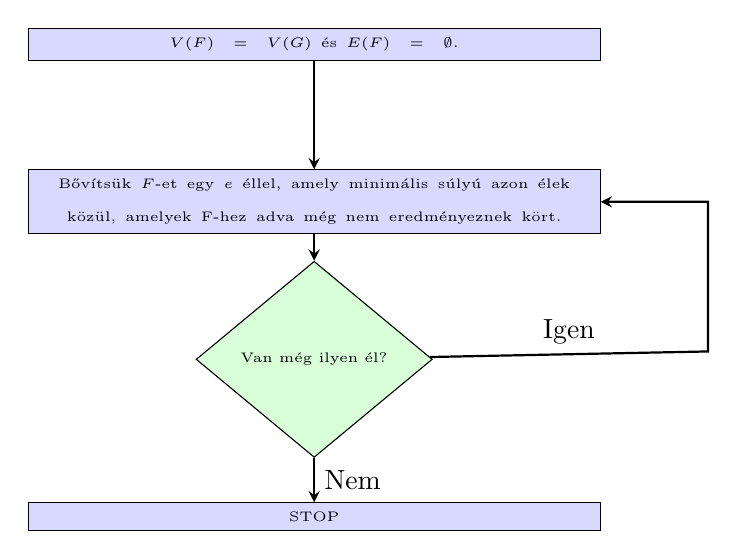
\begin{tikzpicture}[node distance = 2cm, auto]
    % Place nodes
    \node [block] (step1) {\tiny{$V(F)=V(G)$ és $E(F) = \emptyset$.}};
    \node [block, below of=step1] (step2) {\tiny{Bővítsük $F$-et egy $e$ éllel, amely minimális súlyú azon élek közül, amelyek F-hez adva még nem eredményeznek kört.}};
    \node [decision, below of=step2] (step3) {\tiny{Van még ilyen él?}};
    \node [block, below of=step3] (step4) {\tiny{STOP}};

    \draw [arrow] (step1) -- (step2);
    \draw [arrow] (step2) -- (step3);
	\draw [arrow] (step3) -- node {Nem} (step4);    
    \draw[arrow] (step3) -- node {Igen} + (5, 0.1) |- (step2);
    

\end{tikzpicture}

\end{frame}

\begin{frame}

\begin{block}{Tétel: Erős összefüggőség}
Egy összefüggő gráf akkor, és csak akkor irányítható úgy, hogy erősen összefüggő legyen, ha minden \textbf{éléhez} tartozik rajta áthaladó kör.
\end{block}

\end{frame}

\begin{frame}

\begin{block}{Tétel: Euler formula}
Egy összefüggő síkbeli gráf, amelynek $t$ tartománya van, (a külső tartományt is beleértve), eleget tesz az Euler-formulának:
$$v(G) - e(G) + t = 2$$

\end{block}

\begin{block}{Bizonyítás (Sematikus)}
Tekintsünk egy $k$ kört $G$-ben és egy $e \in E(K)$ élet.\\
Mivel $e$ két tartomány határán van $\implies$ $e$ törlésével két szomszéd régió eggyé válik.

(kép)

$\implies$ az élek, és tartományok száma is eggyel csökken.\\
A formula: $v(G) - e(G) + t = 2$ -> $e(G)$ Az $e(G)$ nél ha kivonunk 1-et: $-(-1) = +1$, A $t$-nél pedig -1 $\implies$ a formula értéke ugyan az marad.\\

Az eltörléseket ismételve előbb-utóbb megkapjuk G egy feszítőfáját. (Tétel, feszítőfa létezése)

Fánál $t = 1$ és az élek száma $v(G) - 1$. $\implies$
$$\implies v(G) - e(G) + t = v(G) - (v(G) - 1) + 1 = 2$$

\end{block}
\end{frame}

\begin{frame}
\begin{block}{Tétel: Síkgráf élszáma}
 Ha $G$ egyszerű, síkba rajzolható gráf, és $v(G) \geq 3$, akkor $$e(G) \leq 3v(G) - 6$$.

\end{block}

\begin{block}{Bizonyítás}
\textbf{1. Eset}\\
TFH $G$ összefüggő.\\
Mivel $v(G) = 3$-ra igaz, ezért tfh (legyen) v(G) > 3.\\
Mivel G egyszeű $\implies$ minden tartományát legalább 3 él határolja. $\implies$\\
$\implies$ legalább 3t élet számoltunk.\\
Mivel az elvágó éleket egyszer számoltuk, a többit kétszer $\implies$ $3t \leq 2e(G)$.\\
Az Euler formulából következik, hogy $$3(e(G) - v(G) + 2) \leq 2e(G) \implies e(G) \leq 3v(G) - 6$$\\
\smallskip
\textbf{2. Eset}\\
TFH $G$ nem összefüggő.\\
Ekkor visszavezetjük az első esetre, élek hozzáadásával.

\end{block}

\end{frame}

\begin{frame}
\begin{block}{Tétel: Minimális fokszáma síkgráfban.}
Ha $G$ egyszerű, síkba rajzolható gráf, akkor $$\delta = \min_{{q \in V(G)}} d(a) \leq 5$$

\end{block}

\begin{block}{Bizonyítás (Indirekt)}
TFH $\delta \geq 6$.
Az általánosság megsértése nélkül feltehetjük, hogy $v(G) \geq 3$.\\
$\sum_{{a \in V(G)}} d(a) = 2e(G)$ (fokok száma = 2 x az élek száma)\\
Mivel $\delta \geq 6 \implies 6v(G) \leq 2e(G)$\\
A síkgráf élszáma tételből következik, hogy:\\
$2e(G) \leq 6v(G) - 12   / *2$\\
$6v(G) \leq 6v(G) - 12$ $\rightarrow$ Ellentmondás!

\end{block}

\end{frame}

\begin{frame}
\begin{block}{Tétel: Kuratovszki gráfok}
A Kuratovszki gráfok ($K_5$ és $K_{3,3}$) Nem rajzolhatók síkba.\\
TODO: kép

\end{block}

\begin{block}{Bizonyítás (Indirekt)}
TFH $K_5$ és $K_{3,3}$ síkbarajzolható.\\
\smallskip
\textbf{$K_{3,3}$ esetén}:\\
$v(G) = 6$, és $e(G) = 9$\\
Euler forumlából következik, hogy $t = 5$.\\
Viszont $K_{3,3}$ nem tartalmaz háromszöget, és nincs szeparáló éle. $\implies$\\
$\implies$ $4t \leq 2e(G) \implies 20 \leq 18$. $\rightarrow$ Ellentmondás!\\
\smallskip
\textbf{$K_5$ esetén}:\\
$v(G) = 5$ és $e(G) = 10$\\
Alkalmazzuk a síkgráf élszáma tételt ($e(G) \leq 3v(G) - 6$), ekkor\\
$10 \leq 9$ $\rightarrow$ Ellentmondás!

\end{block}

\end{frame}

\begin{frame}
\begin{block}{Tétel: Kuratovszki tétel}
Egy egyszerű véges gráf \textbf{akkor, és csak akkor} rajzolható síkba, ha nem tartalmaz a Kuratovszki gráfok valamelyikével topologikusan izomorf részgráfot.

\end{block}

\end{frame}

% --------------------  FORÁLIS NYELVEK, ÉS AUTOMATÁK --------------------

\begin{frame}[plain]
\begin{tikzpicture}[overlay, remember picture]
\node[anchor=center] at (current page.center) {
\begin{beamercolorbox}[center]{title}
    {\Huge Formális nyelvek, és Automaták}
\end{beamercolorbox}};
\end{tikzpicture}
\end{frame}

\begin{frame}
\begin{block}{Tétel: Kleene tétel}
Egy nyelv akkor, és csak akkor felismerhető, ha reguláris.

\end{block}

\end{frame}

\begin{frame}
\begin{block}{Tétel: Felismerhető nyelvek komplementere}
$L$ Felismerhető $\implies$ $\overline{L}$

\end{block}

\begin{block}{Bizonyítás}
Legyen $M = (Q, \Sigma , \delta , q_0, F)$ véges automata és $L = L(M)$ (M automata felismeri az L nyelvet).\\
Tekintsük a következő konstrukciót:\\
Legyen $\overline{M} = (Q, \Sigma , \delta, q_0, F)$, ahol $\overline{F} = Q - F$.\\
Ekkor  $L(\overline{M}) = \overline{L}$. (Azaz az $\overline{M}$ automata biztosan felismeri az $\overline{L}$ nyelvet.\\ 
(Triviális, mert amit $L$ nem ismer fel, azt ez biztosan, amit $\overline{L}$ felismer, azt pedig ez nem ismeri fel biztosan.

\end{block}

\end{frame}

\begin{frame}
\begin{block}{Tétel: Felismerhető nyelvek komplementere}
$L_1, L_2$ felismerhető $\implies$ $L_1 \cap L_2$

\end{block}

\begin{block}{Bizonyítás}
Legyen: $L_1 = L(M_1), L_2 = L(M_2)$.\\
Legyen: $M_1 = (Q_1, \Sigma , {\delta}_1, q_1, F_1), M_2 = (Q_2, \Sigma , {\delta}_2, q_2, F_2)$.\\
Legyen: $Q = Q_1 x Q_2$
Legyen: $\delta = Q x \Sigma \rightarrow Q$ (Párok lesznek).\\
Legyen: $\delta((s_1, s_2), a) = ({\delta}_1(s_1, a), {\delta}_2(s_2, a))$, $s_1 \in Q_1, s_2 \in Q_2, a \in \Sigma$\\
\smallskip
Legyen: $q_0 = (q_1, q_2)$\\
Legyen: \textbf{$F_{\cap} = F_1 x F_2$}\\
\smallskip
Legyen: $M_{\cap} = (Q, \Sigma , \delta , q_0, F_{\cap})$\\
\smallskip
Ekkor: $L(M_{\cap}) = L_1 \cap L_2$\\
\end{block}

\end{frame}

\begin{frame}
\begin{block}{Tétel: Felismerhető nyelvek egyesítése}
$L_1, L_2$ felismerhető $\implies$ $L_1 \cup L_2$

\end{block}

\begin{block}{Bizonyítás}
Legyen: $L_1 = L(M_1), L_2 = L(M_2)$.\\
Legyen: $M_1 = (Q_1, \Sigma , {\delta}_1, q_1, F_1), M_2 = (Q_2, \Sigma , {\delta}_2, q_2, F_2)$.\\
Legyen: $Q = Q_1 x Q_2$
Legyen: $\delta = Q x \Sigma \rightarrow Q$ (Párok lesznek).\\
Legyen: $\delta((s_1, s_2), a) = ({\delta}_1(s_1, a), {\delta}_2(s_2, a))$, $s_1 \in Q_1, s_2 \in Q_2, a \in \Sigma$\\
\smallskip
Legyen: $q_0 = (q_1, q_2)$\\
Legyen: \textbf{$F_{\cup} = F_1 x F_2$}\\
\smallskip
Legyen: $M_{\cup} = (Q, \Sigma , \delta , q_0, F_{\cup})$\\
\smallskip
Ekkor: $L(M_{\cup}) = L_1 \cup L_2$\\
\end{block}

\end{frame}

\begin{frame}
\begin{block}{Tétel: Nemdeterminisztikus automata}
Minden $M = (Q, \Sigma , \delta , q_0, F)$ véges nemdeterminisztikus automatával felismerhető nyelv, felismerhető véges automatával.

\end{block}

\begin{block}{Bizonyítás}
Tekintsük az $M' = (Q', \Sigma , {\delta}', Q_0, F')$ véges automatát, ahol\\
$Q' = p(Q)$ ($P(Q)$ $\rightarrow$ hatványhalmaz)\\
${\delta}' : p(Q) x \Sigma \rightarrow p(Q)$ (Az állapotok is halmazok!)\\
${\delta}'(X, a) = \widehat{Y}$, $Y = U_{q \in X} \delta(q, a)$\\
$Q_0 = \widehat{\{q_0\}}$\\
$F' = \{X \supseteq Q : X \cap F \neq \emptyset \}$.\\
Ekkor nyilvánvaló, hogy $L(M') = L(M)$.\\
Megjegyzés: Elég lenne $p(Q)$ azon elemeivel számolni, amelyek elérhetők $Q_0$-ból.

\end{block}

\end{frame}

\begin{frame}
\begin{block}{Tétel: Felismerhető nyelvek szorzata}
$L_1, L_2$ felismerhető $\implies$ $L_1 * L_2$

\end{block}

\begin{block}{Bizonyítás}
Legyen: $L_1 = L(M_1), L_2 = L(M_2)$.\\
Legyen: $M_1 = (Q_1, \Sigma , {\delta}_1, q_1, F_1), M_2 = (Q_2, \Sigma , {\delta}_2, q_2, F_2)$.\\
Legyen: $Q_1 \cap Q_2 = \emptyset$, $L(M_1) = L_1, L(M_2) = L_2$.\\
\bigskip
Legyen: ${\delta}(q, a) = $
$
\begin{cases}
{\delta}_1(q, a) & q \in Q_1 - F_1\\
{\delta}_1(q, a) & q \in F_1, a \neq \epsilon \\
{\delta}_1(q, a) \cup \{q_2\} & q \in F_1, a = \epsilon \\
{\delta}_1(q, a) & q \in Q_2 \\
\end{cases}
$\\
\bigskip
Legyen: $M_1 * M_2 = (Q_1 \cup Q_2, \Sigma , \delta , q_1, F_2)$\\
\bigskip
Ekkor: \textbf{$L(M_1 * M_2) = L_1 * L_2$}\\
\end{block}

\end{frame}

\begin{frame}
\begin{block}{Tétel: Felismerhető nyelvek iterációja}
$L$ felismerhető $\implies$ $L*$ is felismerhető.

\end{block}

\begin{block}{Bizonyítás}
Legyen: $M = (Q, \Sigma , {\delta}, q_0, F)$.\\
Legyen: $M* = (Q \cup \{s_0\}, \Sigma , {\delta}_*, s_0, F \cup \{s_0\})$.\\
\bigskip
Legyen: ${\delta}(q, a) = $
$
\begin{cases}
{\delta}(q, a) & q \in Q $ és $q \notin F\\
{\delta}(q, a) & q \in F$ és $a \neq \epsilon \\
{\delta}(q, a) \cup \{q0\} & q \in F$ és $a = \epsilon \\
\{q_0\} & q = s_0$ és $a = \epsilon \\
\emptyset & q = s_0$ és $a \neq \epsilon \\
\end{cases}
$\\
\bigskip
\textbf{Ekkor: $L(M*) = L*$}\\
\end{block}

\end{frame}

\begin{frame}
\begin{block}{Tétel: Pumpáló lemma reguláris nyelvre}
Minden $L \subseteq {\Sigma}*$ reguláris nyelvhez létezik olyan $p$ természetes szám, amelyre L minden legalább $p$ hosszúságó $u$ szava felírható $$u = xyz$$\\
alakban úgy, hogy\\
\begin{enumerate}
\item $|y| > 0$
\item $|xy| \leq p$
\item $xy'z \in L$ minden $i \geq 0$ egészre.
\end{enumerate}

\end{block}

\begin{block}{Bizonyítás}
Az L reguláris nyelvhez konstruáljuk meg az $M = (Q, {\Sigma}, {\delta}, q_0, F)$ véges automatát úgy, hogy legyen $p = |Q|$.\\
Ha $u \in L$ és $|u| \geq p \implies$ a $q_0, q_1, ...,q_n (q_i \in Q, i = 0, ..., n)$\\
számítási sorozatra az $u$ szón teljesüljön, hogy\\
\begin{enumerate}
\item $n = |u| \geq p$
\item $q_n \in F$
\item ${\exists}i, j : 0 \leq i < j \leq p$ és $q_i = q_j$
\end{enumerate}
\bigskip
Legyen továbbá:
\begin{itemize}
\item $x$ az $u$ szó $i$ hosszú kezdőszelete
\item $y$ az $x$-et követő $j - i$ hosszú rész-szó
\item $z$ az $u n - j$ hosszú zárószelete 
\end{itemize}
\bigskip
\textbf{Ekkor az $u = xyz$ felbontásra teljesülnek a lemma állításai.}
\end{block}

\end{frame}

\begin{frame}
\begin{block}{Tétel: Példa nemreguláris nyelvre}
Az $L = \{0^n1^n : n \geq 0\} \subseteq \{0, 1\}^*$ nyelv nem reguláris.
\end{block}

\begin{block}{Bizonyítás}
Legyen $p$  tetszőleges, ekkor $u = 0^p1^p$.\\
Tfh $x, y, z$ olyan szavak, amelyekre:\\
$u = xyz, |xy| \leq p, |y| > 0$.\\
Ekkor $xy$ csupa 0-ból áll és $y$ tartalmaz legalább egy 0-t. $\implies$\\
$\implies$ $i \neq 1$ esetén $xy'z \notin L$, mert több 0 lessz benne, mint 1-es! $\implies$\\
$\implies$ Sosem találunk megfelelő $p$-t $\implies$ \textbf{A nyelv nem reguláris.}
\end{block}

\end{frame}


\begin{frame}
\begin{block}{Tétel: Derivációs fák}
Egy $X \in (V \cup {\Sigma}_{\epsilon})$-ből induló derivációs fa, amelynek határa az $u \in {\Sigma}^*$ szó, ami akkor és csak akkor létezik, ha $X {\implies}^* u \in {\Sigma}^*$.
\end{block}

\begin{block}{Tétel: Ekvivalens állítások derivációs fákra}
Legyen $G = (V, {\Sigma}, R, S)$ környezetfüggetlen nyelvtan. Ekkor a következők ekvivalensek az $u \in {\Sigma}^*$ szóra:\\
\begin{enumerate}
\item $u \in L(G)$
\item $S {\implies}^*_l u$
\item Létezik olyan $S$-ből induló derivációs fa, amelynek határa $u$.
\end{enumerate}

\end{block}

\end{frame}

\begin{frame}
\begin{block}{Tétel: Reguláris nyelv környezetfüggetlen}
Minden reguláris nyelv környezetfüggetlen.

\end{block}

\begin{block}{Bizonyítás}

\end{enumerate}

\end{block}

\end{frame}

\end{document}